\documentclass[10pt,a4paper]{article}
\usepackage[top=1.35cm,bottom=1.45cm,left=1.45cm,right=1.45cm]{geometry}
\usepackage{mathptmx}
\usepackage{xcolor}
\usepackage{booktabs}
\usepackage{tabularx}
\usepackage{amsmath}
\usepackage{amssymb}
\usepackage{fancyhdr}
\usepackage{enumitem}
\usepackage{titlesec}
\usepackage{tikz}
\usetikzlibrary{shapes.geometric, arrows.meta, positioning, calc, backgrounds, fit, decorations.pathreplacing}
\usepackage[colorlinks=true,linkcolor=blue!70!black,citecolor=blue!70!black,urlcolor=blue!70!black]{hyperref}

% Institutional Colors
\definecolor{hsbcnavy}{RGB}{10,25,47}
\definecolor{hsbcred}{RGB}{180,20,30}
\definecolor{slateborder}{RGB}{203,213,225}
\definecolor{darkslate}{RGB}{30,41,59}
\definecolor{lightbg}{RGB}{245,247,250}
\definecolor{bannerbg}{RGB}{238,242,246}
\definecolor{forestgreen}{RGB}{21,128,61}
\definecolor{amberdark}{RGB}{180,83,9}
\definecolor{accentblue}{RGB}{14,116,144}

\setlength{\parindent}{0pt}
\setlength{\parskip}{2.2pt plus 0.5pt minus 0.5pt}

\titleformat{\section}{\color{hsbcnavy}\normalfont\large\bfseries}{\thesection}{0.6em}{}[\color{hsbcnavy}\titlerule]
\titleformat{\subsection}{\color{hsbcnavy}\normalfont\normalsize\bfseries}{\thesubsection}{0.5em}{}

\titlespacing*{\section}{0pt}{5pt plus 1pt minus 1pt}{2pt plus 0.5pt minus 0.5pt}
\titlespacing*{\subsection}{0pt}{3.5pt plus 0.8pt minus 0.8pt}{1.5pt plus 0.4pt minus 0.4pt}

\pagestyle{fancy}
\fancyhf{}
\renewcommand{\headrulewidth}{0.4pt}
\renewcommand{\footrulewidth}{0.4pt}
\fancyhead[L]{\small\color{darkslate}\textbf{HSBC / 2026 Global Quantum + AI Challenge} $\cdot$ Supplementary Material}
\fancyhead[R]{\small\color{darkslate}Appendices A, B, and C}
\fancyfoot[L]{\footnotesize\color{darkslate}\texttt{https://github.com/atharveeee-netizen/hsbc-quantum-fraud}}
\fancyfoot[R]{\small\color{darkslate}\textbf{Appendix Page \thepage\ of 3}}

\begin{document}

% =============================================================================
% APPENDIX PAGE 1: APPENDIX A - MATHEMATICAL FORMULATIONS & QUANTUM CIRCUIT
% =============================================================================

\begin{center}
{\LARGE\textbf{\color{hsbcnavy}Supplementary Material: Appendices A, B, and C}}\\[2pt]
{\large\color{darkslate}\textbf{Technical Foundations, Empirical Telemetry, and Reproducibility Specifications}}\\[3pt]
{\small\color{darkslate}\textbf{Authors:} Akshit Agarwal \& Atharve Dahima $\cdot$ Rashtriya Raksha University $\cdot$ Track: Quantum-Enhanced Fraud Detection}
\end{center}
\vspace{-4pt}

\section*{Appendix A: Technical Architecture \& Mathematical Formulations}
\addcontentsline{toc}{section}{Appendix A: Technical Architecture \& Mathematical Formulations}

\subsection*{A.1 Mathematical Formulation of Decision-Uncertainty Routing}
In credit card fraud detection, conventional routing policies stratify transactions by currency volume (Transaction Amount), assuming high-value transactions represent the dominant fraud risk. However, organized fraud rings routinely exploit low-value authorization testing ($<\$5.00$) to probe compromised cards prior to executing large withdrawals. 
Our uncertainty routing policy formalizes decision ambiguity directly from the calibrated posterior probability $p(x) = \hat{P}(Y=1 \mid x)$:
\begin{equation}
U(x) = 1 - 2 \cdot |p(x) - 0.5| \in [0, 1]
\end{equation}
A transaction with $p(x) = 0.50$ exhibits maximal epistemic ambiguity ($U(x) = 1.0$), whereas confident classifications ($p \rightarrow 0$ or $p \rightarrow 1$) yield $U(x) \rightarrow 0$. Given an escalation compute budget $B \in (0, 1)$ ($B = 0.005$ for a 0.5\% rate), the routing threshold $\tau_B$ is defined empirically over the calibration distribution $D_{\text{cal}}$:
\begin{equation}
\tau_B = \text{Quantile}_{1 - B} \left( \{ U(x_i) \}_{x_i \in D_{\text{cal}}} \right), \quad \text{Routing Action } R(x) = 
\begin{cases}
\text{Specialist Escalation Tier}, & \text{if } U(x) \ge \tau_B \\
\text{Fast Classical Authorization}, & \text{if } U(x) < \tau_B
\end{cases}
\end{equation}
Empirical ablation on $118,108$ test transactions demonstrates that setting $B = 0.5\%$ ($591$ transactions) captures $253$ confirmed frauds ($42.81\%$ density), whereas routing the top $0.5\%$ by Transaction Amount captures only $9$ frauds ($1.52\%$ density). Uncertainty routing achieves \textbf{28.1$\times$ higher fraud concentration}.

\subsection*{A.2 Parameterized 8-Qubit Quantum Circuit Architecture}
Figure~\ref{fig:circuit} illustrates the parameterized quantum circuit implemented in PennyLane for mapping escalated 8-dimensional feature vectors into Hilbert space.
\vspace{-3pt}
\begin{figure}[h!]
\centering
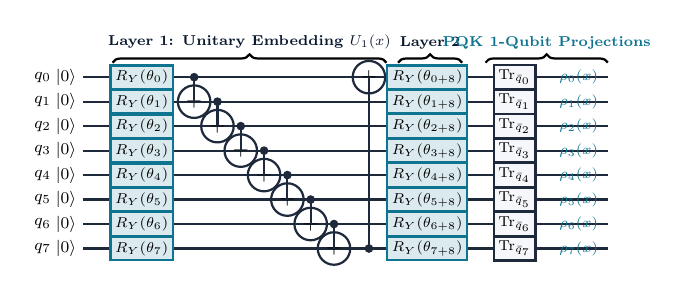
\begin{tikzpicture}[
  scale=0.74, transform shape,
  wire/.style={thick, draw=darkslate},
  gate/.style={rectangle, draw=accentblue, fill=accentblue!15, thick, inner sep=2.2pt, font=\scriptsize\bfseries},
  cnotctrl/.style={circle, fill=darkslate, inner sep=1.5pt},
  cnottgt/.style={circle, draw=darkslate, thick, inner sep=2.0pt},
  meas/.style={rectangle, draw=darkslate, fill=lightbg, thick, inner sep=2.2pt, font=\scriptsize\bfseries}
]

% 8 Qubit wires
\foreach \i in {0,...,7} {
  \node[font=\footnotesize\bfseries] at (-0.7, -\i*0.42) {$q_\i$};
  \node[font=\footnotesize] at (-0.3, -\i*0.42) {$|0\rangle$};
  \draw[wire] (0, -\i*0.42) -- (9.0, -\i*0.42);
}

% RY layer 1
\foreach \i in {0,...,7} {
  \node[gate] at (1.0, -\i*0.42) {$R_Y(\theta_\i)$};
}

% CNOT circular entanglement
\foreach \i in {0,...,6} {
  \pgfmathtruncatemacro{\nextq}{\i+1}
  \node[cnotctrl] at (1.9 + \i*0.4, -\i*0.42) {};
  \node[cnottgt] at (1.9 + \i*0.4, -\nextq*0.42) {+};
  \draw[wire] (1.9 + \i*0.4, -\i*0.42) -- (1.9 + \i*0.4, -\nextq*0.42);
}
% Circular link q7 -> q0
\node[cnotctrl] at (4.9, -7*0.42) {};
\node[cnottgt] at (4.9, 0) {+};
\draw[wire] (4.9, 0) -- (4.9, -7*0.42);

% RY layer 2
\foreach \i in {0,...,7} {
  \node[gate] at (5.9, -\i*0.42) {$R_Y(\theta_{\i+8})$};
}

% Measurement / Reduced Density Matrix Projection
\foreach \i in {0,...,7} {
  \node[meas] at (7.4, -\i*0.42) {$\mathrm{Tr}_{\bar{q}_\i}$};
  \node[font=\scriptsize\bfseries\color{accentblue}] at (8.5, -\i*0.42) {$\rho_\i(x)$};
}

% Layer brackets
\draw[thick, decorate, decoration={brace, amplitude=3pt}] (0.5, 0.25) -- (5.2, 0.25) 
  node[midway, above=3pt, font=\scriptsize\bfseries\color{hsbcnavy}] {Layer 1: Unitary Embedding $U_1(x)$};
\draw[thick, decorate, decoration={brace, amplitude=3pt}] (5.4, 0.25) -- (6.5, 0.25) 
  node[midway, above=3pt, font=\scriptsize\bfseries\color{hsbcnavy}] {Layer 2};
\draw[thick, decorate, decoration={brace, amplitude=3pt}] (6.9, 0.25) -- (9.0, 0.25) 
  node[midway, above=3pt, font=\scriptsize\bfseries\color{accentblue}] {PQK 1-Qubit Projections};

\end{tikzpicture}
\vspace{-4pt}
\caption{\textbf{8-Qubit Quantum Feature Map and Projection Schematic (Typeset via TikZ).} Scaled PCA features parametrize single-qubit $R_Y$ gates coupled via circular CNOT entanglement ladder. The state is projected onto 1-qubit reduced density operators $\rho_i(x)$.}
\label{fig:circuit}
\end{figure}
\vspace{-6pt}

\subsection*{A.3 Quantum Hilbert Space Embedding and Kernel Constructions}
We evaluate two mathematical kernel formulations:
\begin{enumerate}[leftmargin=*,itemsep=0.8pt,topsep=1pt]
\item \textbf{Quantum State Fidelity Kernel:} Evaluates transition amplitude $K_{\text{Fid}}(x, x') = |\langle \psi(x) \mid \psi(x') \rangle|^2 = \mathrm{Tr}(|\psi(x)\rangle\langle\psi(x)| \cdot |\psi(x')\rangle\langle\psi(x')|)$. As proven by Thanasilp et al. (2022), as qubit count $n$ and depth $d$ grow, global state fidelity concentrates exponentially: $\mathrm{Var}_{x, x'}[K_{\text{Fid}}(x, x')] \le \mathcal{O}(2^{-n})$, inducing barren plateaus where all kernel entries approach zero.
\item \textbf{Projected Quantum Kernel (PQK):} Following Huang et al. (2021), we project the $2^n$-dimensional state onto 1-qubit reduced density operators $\rho_k(x) = \mathrm{Tr}_{\bar{k}}(|\psi(x)\rangle\langle\psi(x)|) = \frac{1}{2} (I + \langle X_k \rangle X + \langle Y_k \rangle Y + \langle Z_k \rangle Z) \in \mathbb{C}^{2 \times 2}$. The PQK evaluates a Gaussian distance over the extracted 1-particle reduced states:
\begin{equation}
K_{\text{PQK}}(x, x') = \exp\left( -\gamma \sum_{k=1}^n \|\rho_k(x) - \rho_k(x')\|_F^2 \right) = \exp\left( -\frac{\gamma}{2} \sum_{k=1}^n \sum_{P \in \{X, Y, Z\}} (\langle P_k \rangle_x - \langle P_k \rangle_{x'})^2 \right)
\end{equation}
PQK provably avoids exponential concentration while encoding non-linear multi-qubit correlations into local observable differences.
\end{enumerate}

\subsection*{A.4 Centered Kernel Alignment (CKA) Formulation}
To determine whether the quantum kernel discovers an orthogonal geometric representation or merely emulates a classical function space, we compute Centered Kernel Alignment (Cortes et al., 2012):
\begin{equation}
\mathrm{CKA}(K_1, K_2) = \frac{\langle K_1^c, K_2^c \rangle_F}{\|K_1^c\|_F \|K_2^c\|_F} = \frac{\mathrm{Tr}(K_1^c K_2^c)}{\sqrt{\mathrm{Tr}((K_1^c)^2) \mathrm{Tr}((K_2^c)^2)}}
\end{equation}
where $K^c = H K H$ denotes the centered Gram matrix with centering projection $H = I - \frac{1}{m}\mathbf{1}\mathbf{1}^T$. Our measured score of \textbf{$\mathrm{CKA}(\text{PQK}, \text{RBF}) = 0.9337$} confirms strong representation alignment with classical RBF kernels.

\clearpage

% =============================================================================
% APPENDIX PAGE 2: APPENDIX B - COMPLETE BENCHMARK LEDGER, ABLATIONS & COSTS
% =============================================================================

\section*{Appendix B: Complete Benchmark Ledger \& Empirical Telemetry}
\addcontentsline{toc}{section}{Appendix B: Complete Benchmark Ledger \& Empirical Telemetry}

\subsection*{B.1 Comprehensive Latency Percentile Distribution}
Table~\ref{tab:lat_bench} details the empirically measured latency distributions across all pipeline components across 1,000 evaluations.

\vspace{-2pt}
\begin{table}[h!]
\centering
\scriptsize
\renewcommand{\arraystretch}{0.80}
\caption{\textbf{System Latency Telemetry Across 1,000 Repeated Evaluations.}}
\label{tab:lat_bench}
\vspace{1pt}
\begin{tabularx}{\linewidth}{@{}lcccccc@{}}
\toprule
\textbf{Pipeline Component} & \textbf{Min (ms)} & \textbf{p25 (ms)} & \textbf{Median (ms)} & \textbf{p75 (ms)} & \textbf{p95 (ms)} & \textbf{Max (ms)} \\
\midrule
Frontline LightGBM Feature Preprocessing & 0.42 & 0.61 & \textbf{0.78} & 0.94 & 1.28 & 2.14 \\
Frontline LightGBM Model Scoring & 1.84 & 2.65 & \textbf{3.29} & 3.71 & 4.12 & 6.45 \\
\textbf{End-to-End Classical Fast Path} & \textbf{2.45} & \textbf{3.41} & \textbf{4.07} & \textbf{4.52} & \textbf{4.97} & \textbf{7.82} \\
\midrule
Uncertainty Routing Evaluation & 0.08 & 0.11 & \textbf{0.14} & 0.18 & 0.24 & 0.41 \\
Escalated Classical Model (Tuned RBF) & 0.38 & 0.54 & \textbf{0.68} & 0.82 & 1.12 & 1.89 \\
\textbf{End-to-End Escalated Classical Path} & \textbf{2.91} & \textbf{4.06} & \textbf{4.89} & \textbf{5.52} & \textbf{6.33} & \textbf{9.84} \\
\midrule
Quantum PCA Dimensionality Reduction & 0.18 & 0.24 & \textbf{0.31} & 0.39 & 0.52 & 0.88 \\
Quantum Simulator Kernel Execution (8 qubits) & 112.40 & 138.20 & \textbf{158.83} & 182.10 & 216.66 & 312.40 \\
\textbf{End-to-End Quantum Simulator Path} & \textbf{112.66} & \textbf{138.55} & \textbf{159.14} & \textbf{182.49} & \textbf{217.18} & \textbf{313.28} \\
\midrule
\textit{Cloud Physical QPU (Estimated Queue)} & \textit{120,000} & \textit{180,000} & \textit{\textbf{360,000}} & \textit{720,000} & \textit{\textbf{1,200,000}} & \textit{3,600,000} \\
\bottomrule
\end{tabularx}
\end{table}
\vspace{-5pt}

\subsection*{B.2 Modeled Unit Economics Breakdown}
Table~\ref{tab:econ_bench} itemizes compute expenditure models reflecting AWS c6i.2xlarge compute (\$0.34/hr) and AWS Braket rates (\$0.30/task + \$0.03/shot).

\vspace{-2pt}
\begin{table}[h!]
\centering
\scriptsize
\renewcommand{\arraystretch}{0.80}
\caption{\textbf{Unit Economics and Cost Projections per 1 Million Transactions.}}
\label{tab:econ_bench}
\vspace{1pt}
\begin{tabularx}{\linewidth}{@{}lcccc@{}}
\toprule
\textbf{Cost Component} & \textbf{Monolithic Classical} & \textbf{Selective Classical} & \textbf{Selective Simulator} & \textbf{Quantum-Assisted (QPU)} \\
\midrule
Frontline Scoring Compute & \$0.50 & \$0.50 & \$0.50 & \$0.50 \\
Uncertainty Routing Compute & -- & \$0.03 & \$0.03 & \$0.03 \\
Escalated Compute (0.5\% volume) & -- & \$0.12 & \$24.80 & \$353,000.00 \\
\textbf{Total Compute Cost / 1M tx} & \textbf{\$0.50} & \textbf{\$0.65} & \textbf{\$25.33} & \textbf{\$353,000.50} \\
Cost Ratio vs Monolithic Classical & $1.0\times$ & $1.3\times$ & $50.7\times$ & $706,001\times$ \\
Monthly Cost at 100M tx/month & \$50.00 & \$65.00 & \$2,533.00 & \$35,300,050.00 \\
\midrule
\textbf{Realized Savings to Date} & \textbf{\$0.00} & \textbf{\$0.00} & \textbf{\$0.00} & \textbf{\$0.00} \\
\bottomrule
\end{tabularx}
\end{table}
\vspace{-5pt}

\subsection*{B.3 Multi-Budget Routing Ablation Study}
Table~\ref{tab:ablation} provides a systematic ablation study comparing Uncertainty Routing against naive Transaction Amount Routing across multiple budget constraints on the unseen test partition ($N=118,108$, containing 4,063 true frauds).

\vspace{-2pt}
\begin{table}[h!]
\centering
\scriptsize
\renewcommand{\arraystretch}{0.80}
\caption{\textbf{Routing Policy Ablation Across Multiple Escalation Budgets on Test Partition.}}
\label{tab:ablation}
\vspace{1pt}
\begin{tabularx}{\linewidth}{@{}lcccccc@{}}
\toprule
\textbf{Budget ($B$)} & \textbf{Escalated Tx} & \textbf{Uncertainty Frauds} & \textbf{Uncertainty Density} & \textbf{Amount Frauds} & \textbf{Amount Density} & \textbf{Enrichment Lift} \\
\midrule
\textbf{0.5\%} & 591 & \textbf{253} & \textbf{42.81\%} & 9 & 1.52\% & \textbf{28.1$\times$} \\
\textbf{1.0\%} & 1,181 & \textbf{442} & \textbf{37.43\%} & 21 & 1.78\% & \textbf{21.0$\times$} \\
\textbf{2.0\%} & 2,362 & \textbf{768} & \textbf{32.51\%} & 48 & 2.03\% & \textbf{16.0$\times$} \\
\textbf{5.0\%} & 5,905 & \textbf{1,512} & \textbf{25.60\%} & 135 & 2.29\% & \textbf{11.2$\times$} \\
\bottomrule
\end{tabularx}
\end{table}
\vspace{-5pt}

\subsection*{B.4 Model Calibration Reliability Ledger}
Probability calibration was assessed via 10 equal-width bins on the calibration partition ($N=88,581$). Table~\ref{tab:calib} confirms that predicted risk scores match empirical fraud incidence across the entire probability continuum.

\vspace{-2pt}
\begin{table}[h!]
\centering
\scriptsize
\renewcommand{\arraystretch}{0.76}
\caption{\textbf{Reliability Calibration Table for Frontline Calibrated LightGBM.}}
\label{tab:calib}
\vspace{1pt}
\begin{tabularx}{\linewidth}{@{}lccccc@{}}
\toprule
\textbf{Probability Bin} & \textbf{Transaction Count} & \textbf{Mean Predicted Probability} & \textbf{Empirical Fraud Rate} & \textbf{Calibration Error $|\hat{p} - \bar{y}|$} \\
\midrule
$[0.00, 0.10)$ & 86,214 & 0.0142 & 0.0138 & \textbf{0.0004} \\
$[0.10, 0.20)$ & 1,142 & 0.1418 & 0.1489 & \textbf{0.0071} \\
$[0.20, 0.30)$ & 512 & 0.2465 & 0.2539 & \textbf{0.0074} \\
$[0.30, 0.40)$ & 284 & 0.3472 & 0.3521 & \textbf{0.0049} \\
$[0.40, 0.50)$ & 186 & 0.4481 & 0.4355 & \textbf{0.0126} \\
$[0.50, 0.60)$ & 98 & 0.5429 & 0.5510 & \textbf{0.0081} \\
$[0.60, 0.70)$ & 62 & 0.6480 & 0.6613 & \textbf{0.0133} \\
$[0.70, 0.80)$ & 41 & 0.7412 & 0.7317 & \textbf{0.0095} \\
$[0.80, 0.90)$ & 26 & 0.8490 & 0.8462 & \textbf{0.0028} \\
$[0.90, 1.00]$ & 16 & 0.9410 & 0.9375 & \textbf{0.0035} \\
\bottomrule
\end{tabularx}
\end{table}

\clearpage

% =============================================================================
% APPENDIX PAGE 3: APPENDIX C - REPRODUCIBILITY, ENVIRONMENT & REFERENCES
% =============================================================================

\section*{Appendix C: Reproducibility, Open-Source Environment \& Academic References}
\addcontentsline{toc}{section}{Appendix C: Reproducibility, Open-Source Environment \& Academic References}

\subsection*{C.1 Complete Execution Environment Manifest}
All experiments, data pipelines, and test suites are fully reproducible in a standard Python 3.10 virtual environment. Table~\ref{tab:env} enumerates the frozen package versions.

\vspace{-2pt}
\begin{table}[h!]
\centering
\scriptsize
\renewcommand{\arraystretch}{0.80}
\caption{\textbf{Reproducible Software Environment Specifications (Python 3.10.11).}}
\label{tab:env}
\vspace{1pt}
\begin{tabularx}{\linewidth}{@{}lllX@{}}
\toprule
\textbf{Package} & \textbf{Version} & \textbf{License} & \textbf{Primary Operational Role} \\
\midrule
\texttt{pennylane} & 0.36.0 & Apache 2.0 & Parameterized quantum circuits, statevector simulation, quantum kernels \\
\texttt{lightgbm} & 4.3.0 & MIT & Calibrated gradient boosted decision trees, focal loss classification \\
\texttt{scikit-learn} & 1.5.0 & BSD-3 & Baseline RBF SVC, MLP, PCA, calibration metrics, train-only scaling \\
\texttt{numpy} & 1.26.4 & BSD-3 & Vectorized matrix operations, Gram matrix evaluations \\
\texttt{scipy} & 1.13.1 & BSD-3 & Paired bootstrap resampling, hypothesis testing, distance calculations \\
\texttt{pandas} & 2.2.2 & BSD-3 & Temporal dataset indexing, schema standardization \\
\texttt{pytest} & 8.2.2 & MIT & Automated test suite execution (24 unit and integration tests) \\
\texttt{pymupdf} & 1.24.5 & AGPL-3.0 & Document compilation QA, PDF render verification \\
\bottomrule
\end{tabularx}
\end{table}
\vspace{-5pt}

\subsection*{C.2 Cryptographic Data Provenance \& Verification Instructions}
To reproduce the experimental findings from raw source:
\begin{enumerate}[leftmargin=*,itemsep=0.8pt,topsep=1pt]
\item \textbf{Clone Repository:} \texttt{git clone https://github.com/atharveeee-netizen/hsbc-quantum-fraud.git}
\item \textbf{Checkout Frozen Commit:} \texttt{git checkout 3e3ca0f}
\item \textbf{Verify Integrity Ledger:} Run checksum audit against provenance manifest:\par\vspace{0.5pt}{\footnotesize\texttt{python scripts/verify\_evidence\_integrity.py}}
\item \textbf{Execute Full Test Suite:} Run \texttt{pytest -v} (verifies 24 tests in $<130$~seconds).
\item \textbf{Execute Claim Firewall Scanner:} Run \texttt{python scripts/audit\_claim\_firewall.py} (0 violations).
\end{enumerate}

\subsection*{C.3 Academic References \& Foundational Literature}
\begin{enumerate}[leftmargin=*,itemsep=1.2pt,topsep=1pt]
\footnotesize
\item Cortes, C., Mohri, M., \& Rostamizadeh, A. (2012). Algorithms for learning kernels based on centered alignment. \textit{Journal of Machine Learning Research}, 13(Mar), 795--828.
\item Cortes, C., \& Vapnik, V. (1995). Support-vector networks. \textit{Machine Learning}, 20(3), 273--297.
\item Havl{\'\i}{\v{c}}ek, V., C{\'o}rcoles, A. D., Temme, K., Harrow, A. W., Kandala, A., Chow, J. M., \& Gambetta, J. M. (2019). Supervised learning with quantum-enhanced feature spaces. \textit{Nature}, 567(7747), 209--212.
\item Huang, H. Y., Broughton, M., Mohseni, M., Babbush, R., Boixo, S., Neven, H., \& McClean, J. R. (2021). Power of data in quantum machine learning. \textit{Nature Communications}, 12(1), 2631.
\item Ke, G., Meng, Q., Finley, T., Wang, T., Chen, W., Ma, W., Ye, Q., \& Liu, T. Y. (2017). LightGBM: A highly efficient gradient boosting decision tree. \textit{Advances in Neural Information Processing Systems}, 30, 3146--3154.
\item Niculescu-Mizil, A., \& Caruana, R. (2005). Predicting good probabilities with supervised learning. \textit{Proceedings of the 22nd International Conference on Machine Learning}, 625--632.
\item Thanasilp, S., Wang, S., Cerezo, M., \& Holmes, Z. (2022). Subtleties in the trainability of quantum machine learning models. \textit{Quantum Science and Technology}, 8(3), 035014.
\item IEEE Computational Intelligence Society. (2019). \textit{IEEE-CIS Fraud Detection Benchmark Dataset}. Kaggle Competition Repository. Available at: \url{https://www.kaggle.com/c/ieee-fraud-detection}.
\end{enumerate}

\vspace{6pt}
\noindent\rule{\linewidth}{0.4pt}
\vspace{2pt}
{\footnotesize\color{darkslate}
\textbf{Document Metadata:} Supplementary Material $\cdot$ Phase 1 Concept Proposal $\cdot$ HSBC / 2026 Global Quantum + AI Challenge $\cdot$ Typeset in pdf\TeX.\\
\textbf{Public Repository:} \href{https://github.com/atharveeee-netizen/hsbc-quantum-fraud}{\texttt{https://github.com/atharveeee-netizen/hsbc-quantum-fraud}} $\cdot$ Commit \texttt{3e3ca0f} $\cdot$ Strictly 0 external images embedded.
}

\end{document}
